\section{}
% Flow separates at a sharp corner along a wall and forms a recirculating 
% separation bubble as sketched below (streamlines are shown). The value of the 
% stream function at the wall is zero, and that of the uppermost streamline shown is 
% some positive value ψupper.
% Discuss the value of the stream function inside the separation bubble. In 
% particular, is it positive or negative? Why? Where in the flow is ψ a minimum?


Flow separates at a sharp corner along a wall and forms a recirculating separation bubble as sketched below (streamlines are shown). The value of the stream function at the wall is zero, and that of the uppermost streamline shown is some positive value $\psi_{\text{upper}}$. Discuss the value of the stream function inside the separation bubble. In particular, is it positive or negative? Why? Where in the flow is $\psi$ a minimum?

\begin{figure}[h]
    \centering
    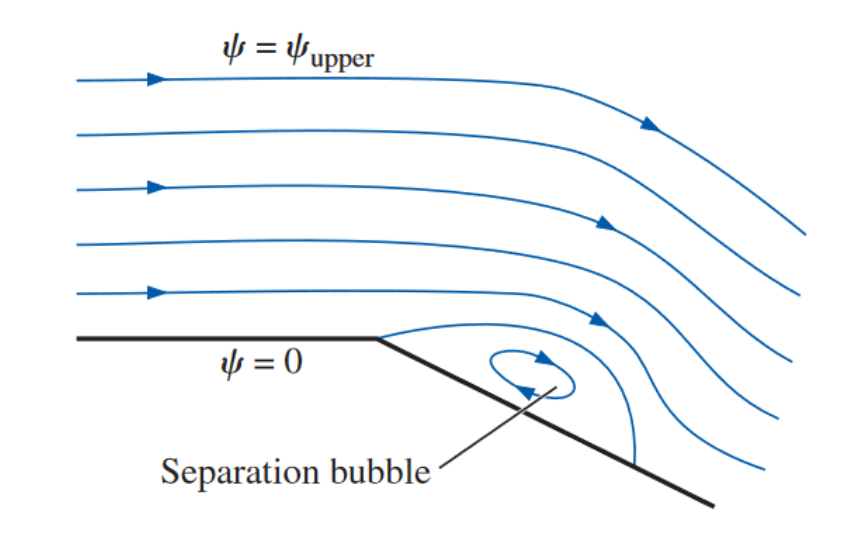
\includegraphics[width=0.5\textwidth]{Questions/Figures/q6 problem diagram.png}
    \caption{Flow separation}
\end{figure}

\subsection*{Solution}
Notice from the figure that the $\Phi = 0$ streamline forms the top of the separation bubble. Since the difference of stream function between two streamlines is equal to the mass flow rate. Since the mass flow rate between the top of the bubble and the streamline shown is positive, the stream function inside the bubble must be \textbf{negative}.

The minimum value of the stream function occurs at the center of the separation bubble, where the mass flow rate is zero. Thus, the stream function will have the most negative value at the \textbf{center} of the separation bubble.